


\documentclass[12pt,a4paper]{report}
\usepackage{etex}
\usepackage{ragged2e}
\usepackage{amsmath}
\usepackage{amssymb}
\usepackage{blindtext}
\usepackage[pdftex]{graphicx} %for embedding images
\usepackage{url} %for proper url entries
\usepackage[a4paper,left=1.5in,right=1.25in,top=1in,bottom=1.25in]{geometry}
\usepackage{titlesec}
\usepackage{setspace}
% Define a new chapter format with a 2-inch top margin
\titleformat{\chapter}[display]
  {\normalfont\huge\bfseries} % Format (bold, large font)
  {\chaptername\ \thechapter} % Chapter number
  {20pt} % Space between number and title
  {}

\titlespacing*{\chapter}{0pt}{2in}{1cm} % (Left, top, bottom spacing)

\titlespacing{\chapter}{0pt}{0pt}{24pt} 
\titlespacing{\section}{0pt}{12pt}{6pt}  
\titlespacing{\subsection}{0pt}{10pt}{5pt}  
\titlespacing{\subsubsection}{0pt}{8pt}{4pt} 
\renewcommand{\baselinestretch}{1.5}




% \usepackage[bookmarks, colorlinks=false, pdfborder={0 0 0}, pdftitle={\texttt{<}pdf title here\texttt{>}}, pdfauthor={\texttt{<}author's name here\texttt{>}}, pdfsubject={\texttt{<}subject here\texttt{>}}, pdfkeywords={\texttt{<}keywords here\texttt{>}}]{hyperref} %for creating links in the pdf version and other additional pdf attributes, no effect on the printed document
%\usepackage[final]{pdfpages} %for embedding another pdf, remove if not required

\usepackage[colorlinks=false, pdfborder={0 0 0}]{hyperref} % Simplified options to reduce memory usage


\begin{document}
\renewcommand\bibname{References} %Renames "Bibliography" to "References" on ref page



%include other pages
\begin{titlepage}

\begin{center}



% Title
\Large \textbf {Title of Seminar Report}\\[0.3in]

\textup{\textsbf{\bf Seminar Report}} \\[0.3in]
\textwidth {\textbf{Submitted by} } \\[0.1in]
\textup{\textbf{Your Name}} \\[0.1in]
\small \textit{in partial fulfilment of the requirements for the award of the degree of} \\[0.25in]
\large \textbf{Bachelor of Technology}\\[0.1in]
\textit{in}\\[0.1in]
\large \textbf\bf {Mechanical/Production Engineering}\\[0.1in]
\vspace{.1in}
  
\vfill

% Bottom of the page

\includegraphics[width=1.16in]{nitc-logo}\\[0.1in]
\Large{Department of Mechanical Engineering}\\
\normalsize
\textsc{National Institute of Technology Calicut}\\
NIT Campus P.O, Calicut,\\
Kerala, India -- 673 601 \\
\vspace{0.3cm}
April 2022

\end{center}

\end{titlepage}

% \cleardoublepage
% %\pagebreak
% % \phantomsection
% % \addcontentsline{toc}{chapter}{Acknowledgements}

\chapter*{\centering \textbf{\MakeUppercase{ACKNOWLEDGEMENT}}}
Students have the freedom to decide, whether acknowledgement is to be given or 
not.  However, it is recommended to give acknowledgements according to the 
standard practice. 
It shall be a single page write-up in paragraph format containing a maximum of 
200 words. 
Proper acknowledgement shall be given to any external agency, which has 
significantly contributed (funding or by any other means) to the work carried out 
for the seminar report. 

\begin{FlushRight}
% Add Team Member Details
\hfill \textbf{Student Name}\\[0.001cm]

\end{FlushRight}




\newpage

% \thispagestyle{empty}

% \begin{center}

% \emph{\huge Certificate}\\[2.5cm]
% \end{center}
\chapter*{\centering \textbf{\MakeUppercase{CERTIFICATE}}}
\justifying
\normalsize This is to certify that the report entitled  \textbf{\textit{ "Title of seminar Report"}} is a bonafide record of the Seminar presented by \textbf{ Name \textit{ (RollNumber)}} in partial fulfillment of the requirements for the award of the degree of \bf{Bachelor of Technology in Mechanical Engineering from National Institute of Technology Calicut}.\\[1.0cm]    

% Bottom of the page
\begin{flushright}
\texttt{}\bf{Faculty in Charge}\texttt{}\\
(ME3099 - Seminar)\\
\emph{Dept. of Mechanical Engineering}\\[1.5cm]

\textbf{Professor and Head}\\
\emph{Dept. of Mechanical Engineering}
\end{flushright}

\begin{flushleft}
Place: NIT Calicut\\
\vspace{1.0}
Date: DD Month YYYY
\end{flushleft}




\chapter*{\centering \textbf{\MakeUppercase{ABSTRACT}}}

 
Abstract shall be a one-page (maximum one page)) write-up giving the summary 
of the seminar report. 
It shall be written in paragraph format (maximum 3 or 4 paragraphs) containing 
approximately 200 words. 
The abstract generally contains the significance of the work, objectives, 
methodology and the major findings. 
Keep in mind that, it is from the abstract, the reader decides about the relevance 
of the work to him, and whether to go ahead with reading the report. 




\clearpage % Ensures that numbering starts on a fresh page
\pagenumbering{roman} %numbering before main content starts
\chapter*{List of Abbreviations}
\addcontentsline{toc}{chapter}{List of Abbreviations}

\begin{tabbing}
    \hspace{2cm} \= \hspace{5cm} \= \kill
    AI \> Artificial Intelligence \\
    ML \> Machine Learning \\
    NLP \> Natural Language Processing \\
\end{tabbing}


% Add List of Symbols
\chapter*{List of Symbols}
\addcontentsline{toc}{chapter}{List of Symbols}
\begin{tabbing}
    \hspace{2cm} \= \hspace{5cm} \= \kill
    $\alpha$ \> Alpha (Coefficient) \\
    $\beta$ \> Beta (Regression Coefficient) \\
    $\sum$ \> Summation \\
\end{tabbing}


% Add List of Figures
\listoffigures
 \addcontentsline{toc}{chapter}{List of Figures}

% Add List of Tables
\listoftables
\addcontentsline{toc}{chapter}{List of Tables}

\renewcommand{\contentsname}{\centering\vspace{-1cm}Contents}
\renewcommand{\baselinestretch}{0.35} % Reduce only ToC spacing

% Now, add the Table of Contents
\tableofcontents


\newpage
\pagenumbering{arabic} %reset numbering to normal for the main content
\chapter{\centering \textbf{\MakeUppercase{INTRODUCTION}}}
\justifying
\section{Preamble}
[Add Your Preamble]

\section{Problem Definition}
[Add Content here]

\section{Outline of the Report}
[Add Content here] %objective changed to problem definition

\chapter{\centering \textbf{\MakeUppercase{Literature Review}}}

\section{\textbf{\MakeUppercase{Section Heading}}}
[Add your content]

 %literature survey included in this
\chapter{\texorpdfstring{\centering \textbf{\MakeUppercase{Topic Specific Title}}}{Topic Specific Title}}

\section{\textbf{\MakeUppercase{the vacuum cleaner’s task}}}
\justifying
To clean an empty room, two motion trajectories can be used: spiral and zigzag.
The vacuum cleaner robot is tasked with sweeping every accessible area in the entire space while avoiding obstacles. If the robot passes by an area position, it will be cleaned; if it has not been cleaned yet, it will be.
The path planning of the coverage region (PPCR) is a task in which the robot must sweep all available free area while avoiding obstacles with an effective trajectory.
This efficient path should be short in length and contain the fewest number of turning angles and revisiting cells possible.
\section{\texttt{ The environment modeling}}
\justifying
An crucial component of the vacuum cleaner robot's duty must be ensured before it can begin, and that is the modelling of the surroundings.
The environment modeling is based on the workspace map, which is created using sensory data gathered from various sensors such as a camera, an infrared sensor, and an ultrasonic sensor.
To make the robot's movements easier, the workspace is divided into discs in the shape of a cleaning robot rather than rectangles or squares. The diagonal length of a discrete area represented by that disc cell is considered equal to the diameter of a sweeping robot.
Each disc symbolizes an impediment or a free position in the environment for the robot to inhabit. There are a maximum of eight surrounding position jth for each connection.

 \chapter{\centering \textbf{\MakeUppercase{Title of Some Important contents}}}
\justifying
[Small Introduction]
\section{\textbf{\MakeUppercase{Section Title}}}

The global path planning for the coverage region is defined as the path taken by the robot from a start position Ps(x, y) to an exit position Pe(x, y) while passing through all accessible places and avoiding obstacles. To get this global path, partition it into mini-paths, the latter of which must not exceed the sensor's range, as shown in Fig. 4.1.\\
\\\begin{figure}[htb]
\centering
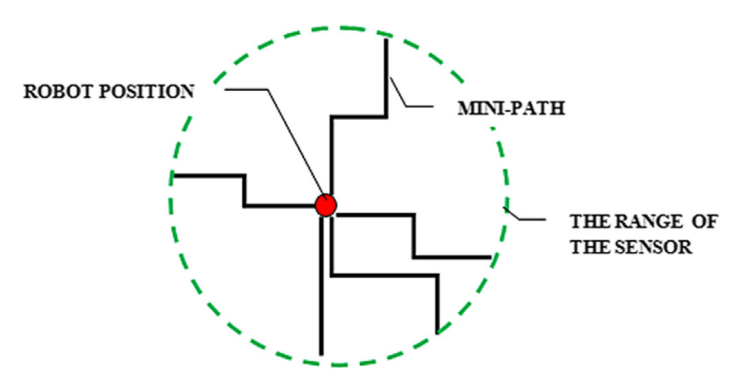
\includegraphics[scale=0.5]{fig4.1.png} % e.g. insert ./image for image.png in the working directory, adjust scale as necessary
\caption{\texttt{}The path planning method\texttt{}}
\label{fig:label} % insert suitable label, this is used to refer to a fig from within the text as shown above
\end{figure}\\

[Add your content and learn how to add images from the example  above]

\chapter{\centering \textbf{\MakeUppercase{Results and Discussion}}}

\section{\textbf{\MakeUppercase{Results}}}
\\Add Content Here\\

\section{\textbf{\MakeUppercase{Analysis}}}
\\Add Content Here\\



\chapter{\texorpdfstring{{}\centering \textbf{\MakeUppercase{Conclusions and Scope for Future Work }}}{Conclusions and Scope for Future Work}}
\justifying

\section{\textbf{\MakeUppercase{Conclusions}}}
Add Content Here
\vspace{2.0pt}\\
\section{\textbf{\MakeUppercase{Scope for Future Work}}}
Add Content Here

\cleardoublepage
%\pagebreak
\phantomsection
\addcontentsline{toc}{chapter}{References}
\begin{thebibliography}{99}

\bibitem{citation-1-name-here}\texttt{}Mohamed Amine Yakoubi, Mohamed Tayeb Laskri, 2016. The path planning of cleaner robot for coverage region using Genetic Algorithms. Journal of Innovation in Digital Ecosystems, Volume 3, Issue 1,2016, Pages 37-43, ISSN 2352-6645\texttt{},\\ 

\bibitem{citation-2-name-here}\texttt{}Tipaldi GD, Meyer-Delius D, Burgard W., 2013. Lifelong localization in changing environments. The International Journal of Robotics Research.;32(14):1662-1678. doi:10.1177/0278364913502830\texttt{},\\ 
\bibitem{citation-3-name-here}\texttt{}Hameed, Ibrahim. 2013. Intelligent Coverage Path Planning for Agricultural Robots and Autonomous Machines on Three-Dimensional Terrain. Journal of Intelligent And Robotic Systems.74. 10.1007/s10846-013-9834-6.\texttt{},\\ 
\end{thebibliography}


\end{document}
